\section{Проектирование и разработка архитектуры программного продукта}

После анализа требований к разрабатываемому продукту нужно составить все необходимые диаграммы, включая MindMap и UseCase.

\subsection{Построение диаграммы связей}

Для общей наглядности внутренностей проекта была составлена карта связей, она же MindMap, показанная на
рисунке \ref{des:mind_map}.

\begin{figure}[H]
    \center{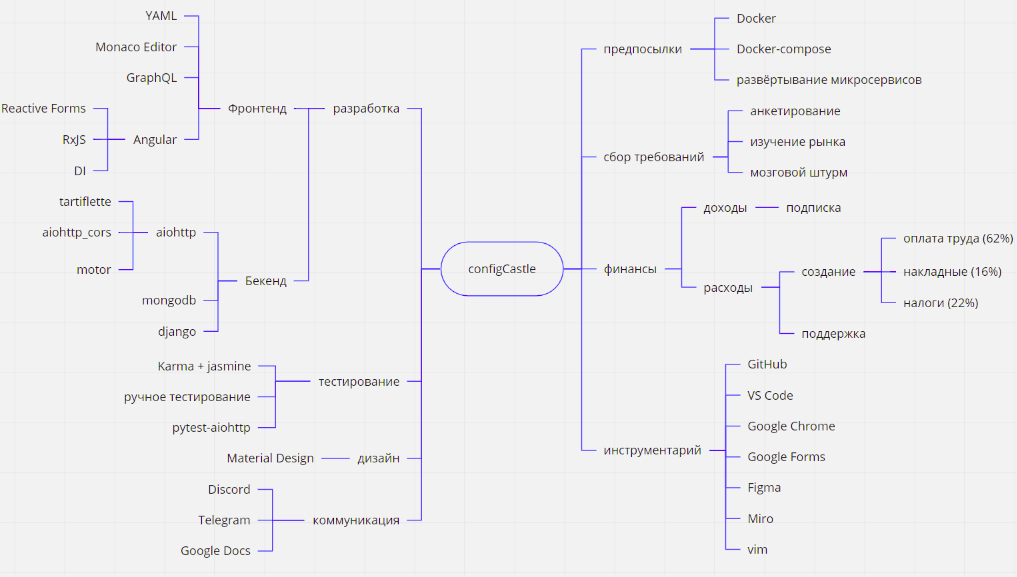
\includegraphics[scale=0.34]{mindmap.png}}
    \caption{Диаграмма связей}
    \label{des:mind_map}
\end{figure}

Здесь показана общая концепция продукта, что стало его предпосылкой, какие инструментальные средства использовались
и так далее.

В дальнейшем можно использовать эту карту, разместив её в wiki проекта для того, чтобы новые разработчики смогли ознакомиться с ней
и приступить к работе с минимальными затратами, понять какую проблему решает продукт, что используется для разработки, как происходит
коммуникация между разработчиками и с какими библиотеками необходимо быть знакомым.

\subsection{Разработка сценария использования}

После анализа ответов на вопрос можно прийти к определённым сценариям взаимодействия с пользователем. Исходя из принципа доступности и легко-понятного
пользовательского интерфейса, можно сконструировать определённые сценарии взаимодействия пользователей с программным продуктом. Результат подобной работы
изображен на так называемой диаграмме UseCase, привидённой на рисунке \ref{des:use_case}.

\begin{figure}[H]
    \center{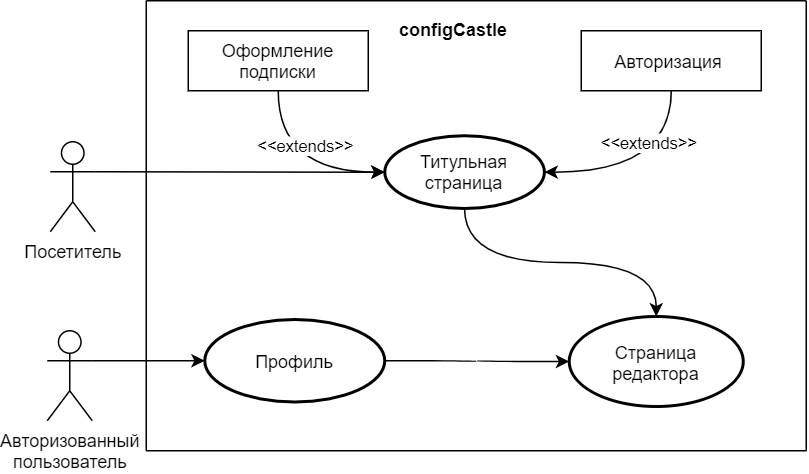
\includegraphics[scale=0.5]{usecase.png}}
    \caption{Диаграмма UseCase}
    \label{des:use_case}
\end{figure}
